\documentclass[
  captions=tableheading,
  bibliography=totoc, 
  titepage=firstiscover,
]{scrartcl}

\usepackage{blindtext} %neuer input

\usepackage{longtable} % Tabellen über mehrere Seiten

\usepackage[utf8]{inputenc} %neuer input

\usepackage{scrhack}

\usepackage[aux]{rerunfilecheck} %Warnung falls nochmal kompiliert werden muss

\usepackage{fontspec} %Fonteinstellungen

\recalctypearea{}

\usepackage[main=ngerman]{babel} %deutsche Spracheinstellung

\usepackage{ragged2e} %neuer input

\usepackage{amsmath, nccmath}

\usepackage{amssymb} %viele mathe Symbole

\usepackage{mathtools} %Erweiterungen für amsmath


\DeclarePairedDelimiter{\abs}{\lvert}{\rvert}
\DeclarePairedDelimiter{\norm}{\lVert}{\rVert}

\DeclarePairedDelimiter{\bra}{\langle}{\rvert}
\DeclarePairedDelimiter{\ket}{\lvert}{\rangle}

\DeclarePairedDelimiterX{\braket}[2]{\langle}{\rangle}{
#1 \delimsize| #2
}

\NewDocumentCommand \dif {m}
{
\mathinner{\symup{d} #1}
}


\usepackage[
  math-style=ISO,
  bold-style=ISO,
  sans-style=italic,
  nabla=upright,
  partial=upright,
  warnings-off={
    mathtools-colon,
    mathtools-overbracket,
  },
]{unicode-math}

\setmathfont{Latin Modern Math}
\setmathfont{XITS Math}[range={scr, bfscr}]
\setmathfont{XITS Math}[range={cal, bfcal}, StylisticSet=1]


\usepackage[
  locale=DE,
  separate-uncertainty=true,
  per-mode=reciprocal,
  output-decimal-marker={,},
]{siunitx}

\usepackage[autostyle]{csquotes} %richtige Anführungszeichen

\usepackage{xfrac}

\usepackage{float}

\floatplacement{figure}{htbp}

\floatplacement{table}{htbp}

\usepackage[ %floats innerhalb einer section halten
  section,   %floats innerhalb er section halten
  below,     %unterhalb der Section aber auf der selben Seite ist ok
]{placeins}

\usepackage[
  labelfont=bf,
  font=small,
  width=0.9\textwidth,
]{caption}

\usepackage{subcaption} %subfigure, subtable, subref

\usepackage{graphicx}

\usepackage{grffile}

\usepackage{booktabs}

\usepackage{microtype} %Verbesserungen am Schriftbild

\usepackage[
backend=biber,
]{biblatex}

\addbibresource{../lit.bib}

\usepackage[ %Hyperlinks im Dokument
  german,
  unicode,
  pdfusetitle,
  pdfcreator={},
  pdfproducer={},
]{hyperref}

\usepackage{bookmark}

\usepackage[shortcuts]{extdash}

%\usepackage{warpcol}


\begin{document}
    \title{V353 Relaxationsverhalten des RC-Kreises}
    \author{  
    Tobias Rücker\\
    \texorpdfstring{\href{mailto:tobias.ruecker@tu-dortmund.de}{tobias.ruecker@tu-dortmund.de}
    \and}{,} 
    Paul Störbrock\\
    \texorpdfstring{\href{mailto:paul.stoerbrock@tu-dortmund.de}{paul.stoerbrock@tu-dortmund.de}}{}
    }
    \date{Durchführung: 19.11.2019, Abgabe: 26.11.2019\vspace{-4ex}}
\maketitle
\center{\Large Versuchsgruppe: \textbf{42}}
    
    \begin{abstract}
        Ziel: 
    \end{abstract}
\newpage
\tableofcontents
\newpage
\justifying
\section{Theorie}
  Als RC-Kreis wird eine Reihenschaltung bestehend aus einem Kondensator 
  und einem Widerstand beschrieben, durch welchen ein Strom I fließt. \\
  Dabei stellt der Kondensator beim Auf- und Entladen einen Relaxationsvorgang dar, 
  was bedeutet, dass die Spannung des Kondensators bei einem Entladevorgang 
  nicht-oszillatorisch zum Anfangszustand zurückkehrt. \\
  Beim Entladevorgang eines Kondensators mit der Kapazität C wird eine Gleichspannung $U_0$ 
  angelegt, die nach dem trennen des Generators über einen Widerstand R abfällt.\\
  Mit der Anfangsbedingung $U_C(0)=U_0$ kann der Entladevorgang beschrieben werden durch \cite{V353}
  \begin{align}
  &U_C(t) = U_0 \cdot e^{-\frac{1}{\tau} t} \quad &\text{mit} \, \tau &= RC  \label{eq:UcEnt} \text{,}
    \intertext{wobei $\tau$ \;Zeitkonstante des Relaxationsvorgangs genannt wird. Sie bestimmt, 
    wie schnell sich das System seinem Endzustand nähert.
    Beim Aufladevorgang sieht die Gleichung mit der Anfangsbedingung $U(0)=0$ 
    folgendermaßen aus \cite{V353}:}
  &U_C(t) = U_0 \, (1-e^{-\frac{1}{\tau} t}) \quad &\text{mit} \, \tau &= RC  \label{eq:UcAuf}
    \intertext{Relaxationsvorgänge sind beim RC-Kreis allerdings nicht auf den Ent- und 
    Aufladevorgang beschränkt. Auch bei einer Wechselspannung lässt sich dieses 
    Verhalten wiederfinden. Bei einer Wechselspannung stellt sich zwischen Strom 
    und Spannung eine frequenzabhängige Phase $\varphi(\nu)$ ein \cite{V353}}
  &\varphi(\nu) = \arctan (-\omega \, RC) \quad &\text{mit} \; \omega &= 2 \pi \nu. \label{eq:nu}
  \end{align}
  Dadurch wird die Phase zwischen $U_C(t)$ und $U(t)$ bei $\omega \ll \sfrac{1}{\tau}$
  noch ungefähr null sein. Bei steigender Frequenz wird die Phasendifferenz immer größer
  bis sie im Unendlichen gegen $\sfrac{\pi}{2}$ geht.
  Die Beziehung zwischen der Amplitude, der Spannung und der Kreisfrequenz lautet dann 
  folgendermaßen \cite{V353}:
  \begin{align}
    A(\omega) &= \frac{U_0}{\sqrt{1 + \omega^2 \, R^2  C^2}} \label{eq:A}
  \end{align}
  Aus \ref{eq:A} ergibt sich eine weitere Eigenschaft des RC-Glieds. Bei niedrigen 
  Frequenzen geht $A(\omega)$ gegen $U_0$. Während es für große Frequenzen
  gegen Null geht.
  Das wird im allgemeinen als Tiefpass bezeichnet und  wird in der 
  elektrischen Schaltungstechnik häufig eingesetzt, um niedrige Frequenzen
  herauszufiltern.\\
  Ein RC-Kreis kann auch unter der Bedingung $\omega \gg \sfrac{1}{RC}$ eine 
  zeitlich veränderliche Spannung $U(t)$ integrieren. Infolgedessen lässt sich 
  zeigen, dass $U_C(t)$ näherungseweise beschrieben werden kann durch \cite{V353}:
  \begin{align}
    U_C(t) &= \frac{1}{RC} \int_0^t{U(t') \, \symup{d}t'}
  \end{align}


\section{Aufgaben}
 \begin{enumerate}
    \item[a)] Zuerst wird die Zeitkonstante $\tau$ eines RC-Glieds durch 
              eine lineare Ausgleichsrechnung bestimmt.

    \item[b)] Dannach wird aus den aufgenommenen Messwerten für Spannung und 
              Frequenz mit einer nicht-linearen Ausgleichsrechnung $\tau$ berechnet 
              und ein zugehöriges $\{ A(\nu _i)/U_0,\nu _i \}$-Diagramm geplottet.
  
    \item[c)] Daraufhin wird der gleiche Prozess aus b) nochmal mit
              $\varphi$ anstelle von $A(\nu _i)/U_0$ durchgeführt.
  
    \item[d)] Zuletzt wird gezeigt, dass ein RC-Kreis unter hohen Frequenzen 
              als Integrator arbeiten kann.
  \end{enumerate}

  



\section{Versuchsaufbau}
Benötigt werden: \textit{ein analoges Zweikanal-Oszilloskop, ein Generator, ein RC-Glied, drei BNC-Kabel, ein BNC-Steckverbinder }\\
Zuerst wird an dem Generatorausgang eine BNC-Steckverbindung angebracht. 
Dann wird der Generator mit dem RC-Glied und dem Oszilloskop verbunden. \\
Zuletzt wird das RC-Glied am zweiten Eingang des Oszilloskop angeschlossen.

\section{Versuchsdurchführung}
\begin{enumerate}
\item[a)] Für die Berechnung von $\tau$ über eine Auf- oder Entladekurve wird der 
          Generator auf eine Rechteckspannung geschaltet und auf einen geeigneten 
          Triggerpegel eingestellt. Daraufhin wird ein Bild von der Auf- 
          oder Entladekurve der Schaltung angefertigt.\\
\item[b)\textbackslash c)] Für den nächsten Teil wird der Generator auf eine Sinusspannung 
          eingestellt. Dabei sollen die Spannungsverläufe von $U_C(t)$ und der 
          Generatorspannung auf dem Oszilloskop gleichzeitig angezeigt werden. 
          Dann werden die Werte für die Amplitude, der Kondensatorspannung 
          [$A(\omega$)] und dem zeitlichen Abstand der Nulldurchgänge 
          [$a$] in Abhängigkeit von der Frequenz über drei Zehnerpotenzen gemessen.\\
\item[d)] Um die Integrierbarkeit nachzuweisen, wird am Generator eine passende 
          Frequenz für die Integration eingestellt. Dannach wird nacheinander eine 
          Rechteck-, Sinus- und Dreiecksschwingung auf das RC-Glied gegeben. 
          Dabei sollen wieder beide Spannungen auf dem Oszilloskop dargestellt 
          werden. Im Anschluss werden dann Fotos von den Oszillogrammen gemacht.
\end{enumerate}

\section{Auswertung}

%Auswertung 4a %%%%%%%%%%%%%%%%%%%%%%%%%%%%%%%%%%%%%%%%%%%%%%%%%%%%%%%%%%%%%%%%%%%%%%%%%%%%%%%%%%%%%%%%%%%%%%%%%
  
  Das Diagramm des Oszilloskops aus dem die Messwerte für die Tabelle \ref{tab:data4a} entnommen 
  wurden, sieht folgendermaßen aus:
  \begin{figure}[H]
    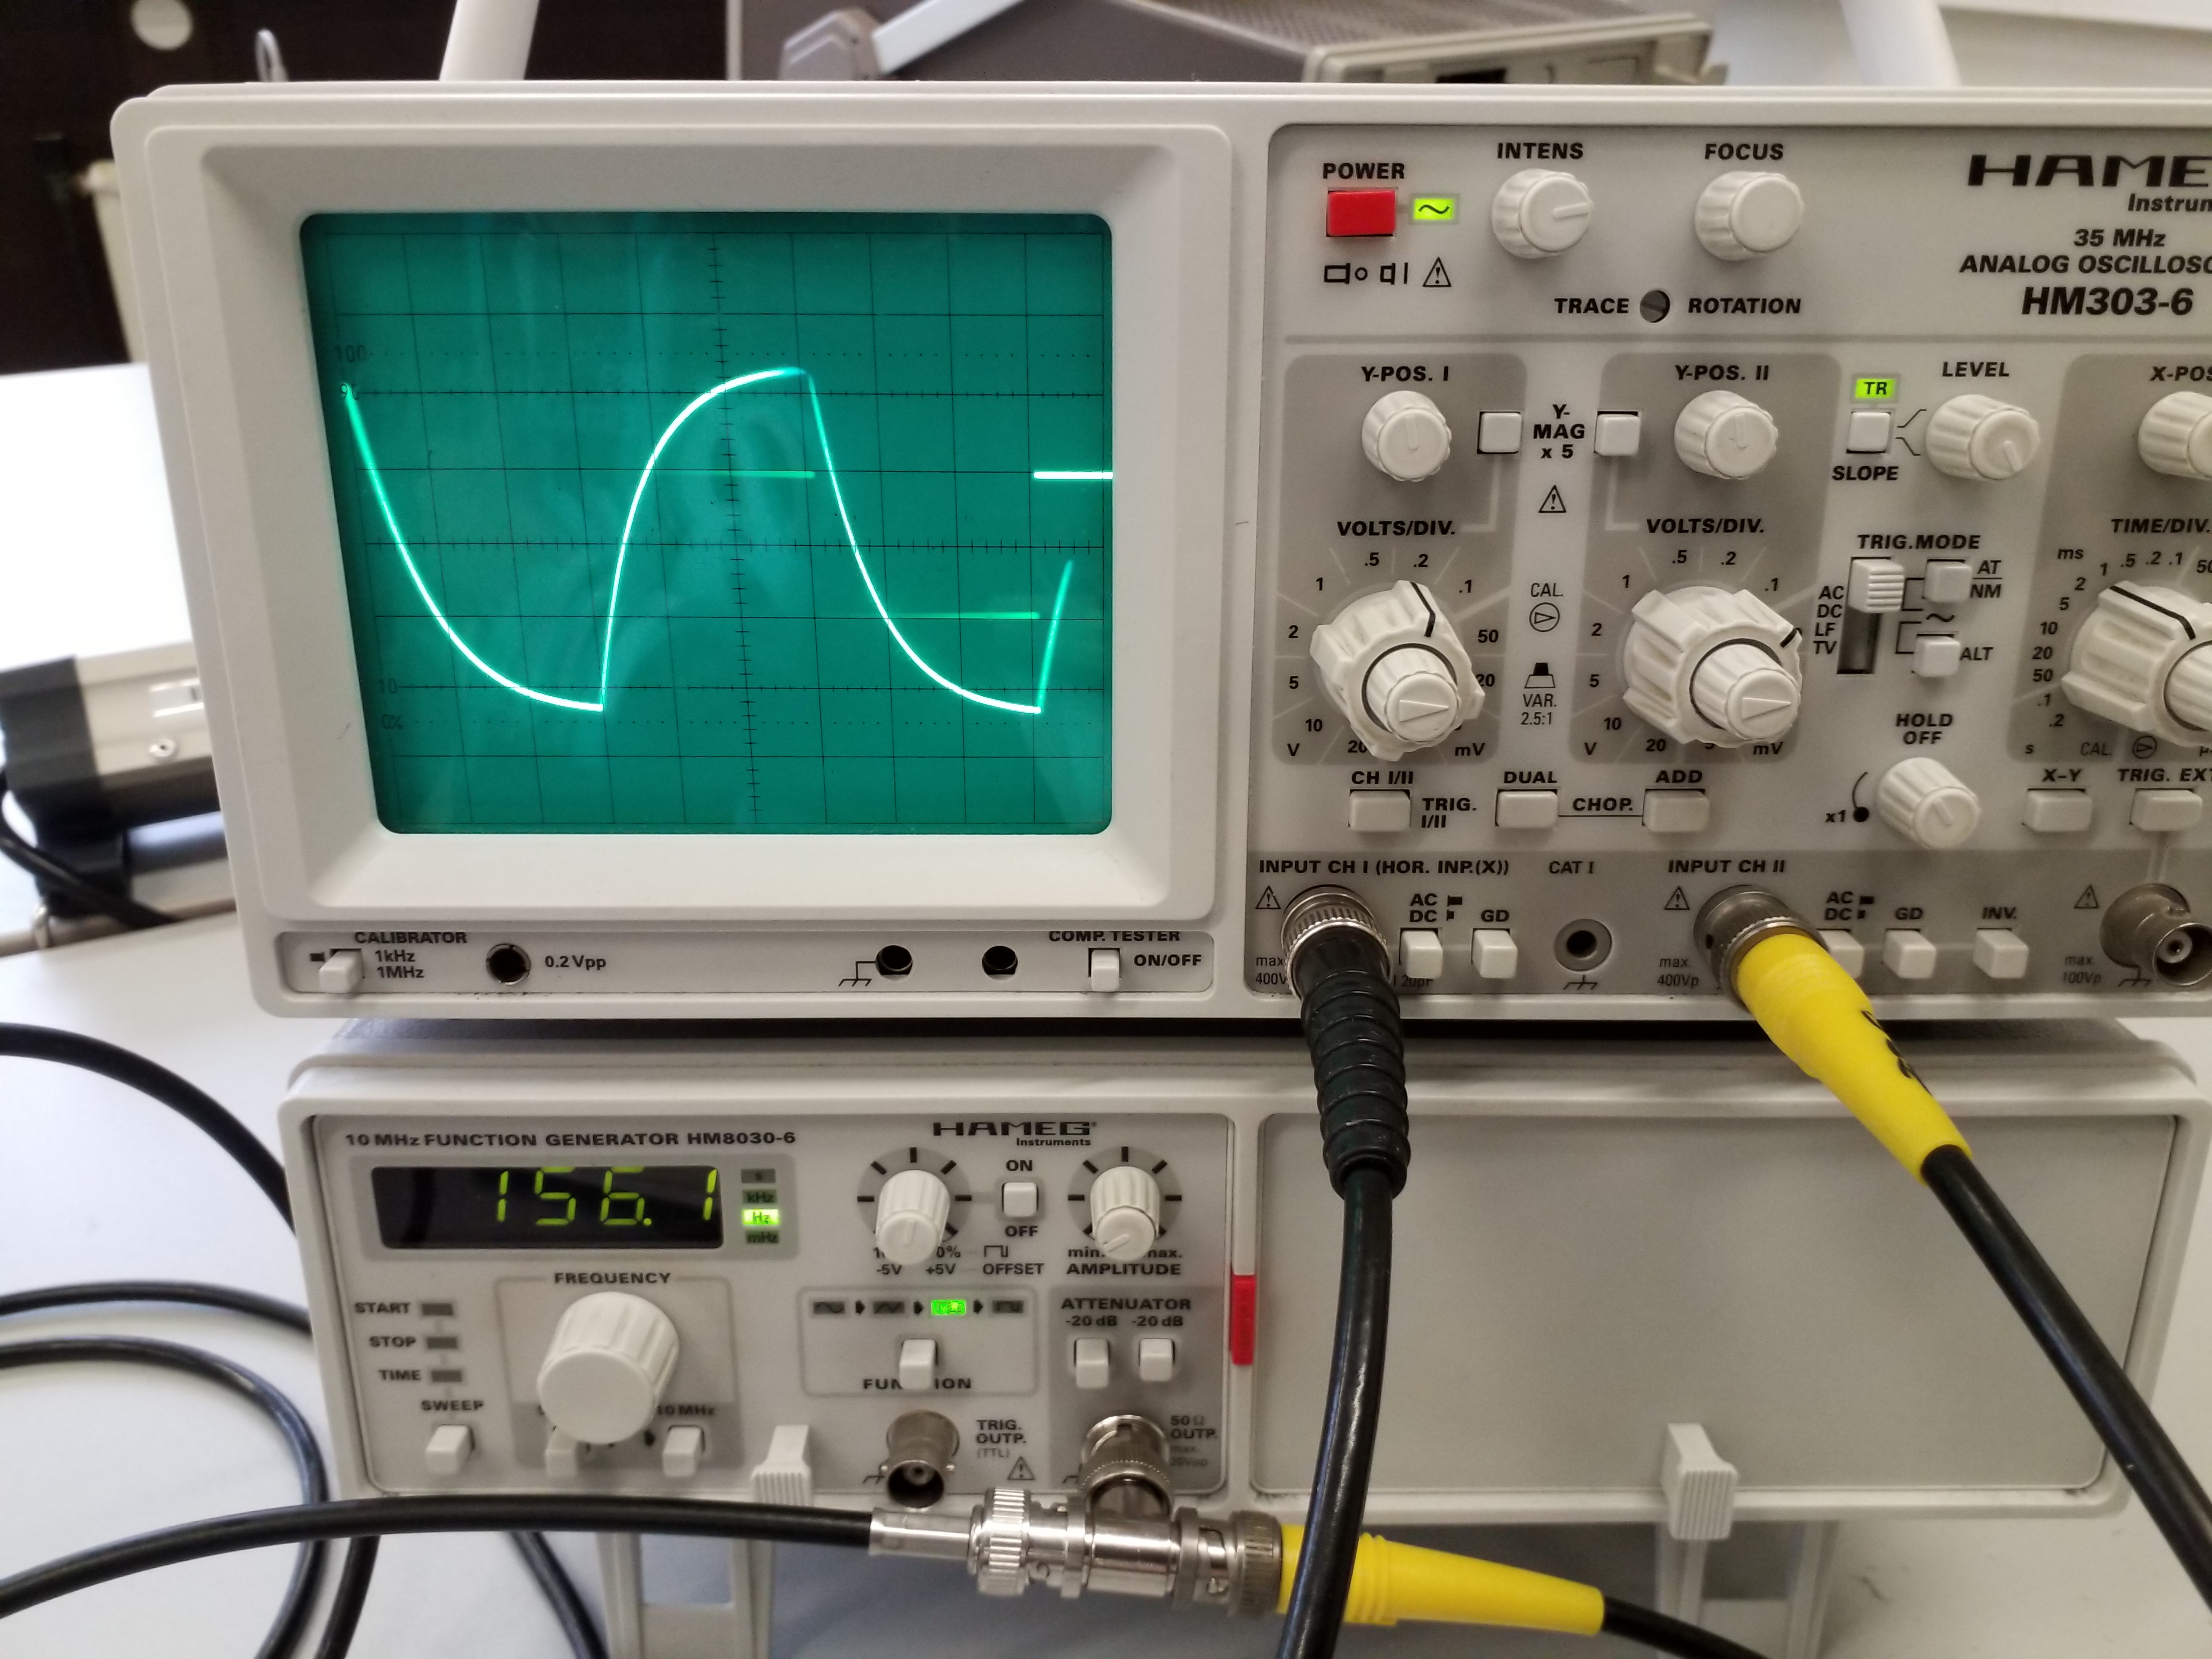
\includegraphics[width=\textwidth]{images/4a.jpg}
    \centering
    \caption{Auf- und Entladekurve des Kondensators}
    \label{fig:4ajpg}
  \end{figure}
  Die Messwerte stammen dabei aus der rechten Entladungskurve.
  \begin{table}[H]
        \centering
        \caption{Messdaten von a)}
        \input{table_4a.tex} 
        \label{tab:data4a}
  \end{table}

  \flushleft{Aus diesen Messwerten wurde dann mithilfe des Programms Scipy} \cite{scipy} und dem Befehl linregress() eine
  Ausgleichsgerade mit den Parametern

  \begin{align*}
    m &= \text{\input{slope.tex}}\\
    b &= \text{\input{intercept.tex}}
  \end{align*}
  berechnet.
  
  \begin{figure}[H]
    \includegraphics[width=\textwidth]{build/plot4a.pdf}
    \centering
    \caption{Lineare Regression von Aufgabe a)}
    \label{fig:4a}
  \end{figure}

  \begin{equation}
  \tau = \text{\input{build/mean_aRC.tex}}
  \end{equation}

% Auswertung 4b %%%%%%%%%%%%%%%%%%%%%%%%%%%%%%%%%%%%%%%%%%%%%%%%%%%%%%%%%%%%%%%%%%%%%%%%%%%%%

  Für die nichtlineare Ausgleichsrechnung aus Aufgaben b) und c) benötigten Messwerte finden sich in der folgenden Tabelle:

  \begin{table}[H]
        \centering
        \caption{Messdaten von b) und c)}
        \input{table_4b.tex} 
        \label{tab:data}
  \end{table}

  Die Werte aus der Tabelle für $\nu$ und $\sfrac{A(\omega)}{U_0}$ wurden in Abbildung \ref{fig:4b} graphisch
  dargestellt. Mithilfe der Formel \ref{eq:A} und dem Befehl curve\_fit() aus Scipy \cite{scipy} wurde 
  die nichtlineare Regressionskurve für Abbildung \ref{fig:4b} berechnet:

  \begin{figure}[H]
    \includegraphics[width=\textwidth]{build/plot4b.pdf}
    \centering
    \caption{Nichtlineare Regression von Aufgabe b)}
    \label{fig:4b}
  \end{figure}

  Aus der curve\_fit() Funktion wird anschließend 

  \begin{equation}
  \tau = \text{\input{build/mean_bRC}}
  \end{equation}

  entnommen.

  % Auswertung 4c %%%%%%%%%%%%%%%%%%%%%%%%%%%%%%%%%%%%%%%%%%%%%%%%%%%%%%%%%%%%%%%%%%%%%%%%%%%%%%%%%%%%%%%%%%%%

  \begin{figure}[H]
    \includegraphics[width=\textwidth]{build/plot4c.pdf}
    \centering
    \caption{Nichtlineare Regression von Aufgabe c)}
    \label{fig:4c}
  \end{figure}

  \begin{equation}
  \tau = \text{\input{build/mean_cRC}}
  \end{equation}

  % Auswertung 4d %%%%%%%%%%%%%%%%%%%%%%%%%%%%%%%%%%%%%%%%%%%%%%%%%%%%%%%%%%%%%%%%%%%%%%%%%%%%%%%%%%%%%%%%%%%%%%%%%%%%%55

  \begin{figure}[H]
  \centering
    \begin{subfigure}{0.48\linewidth}
      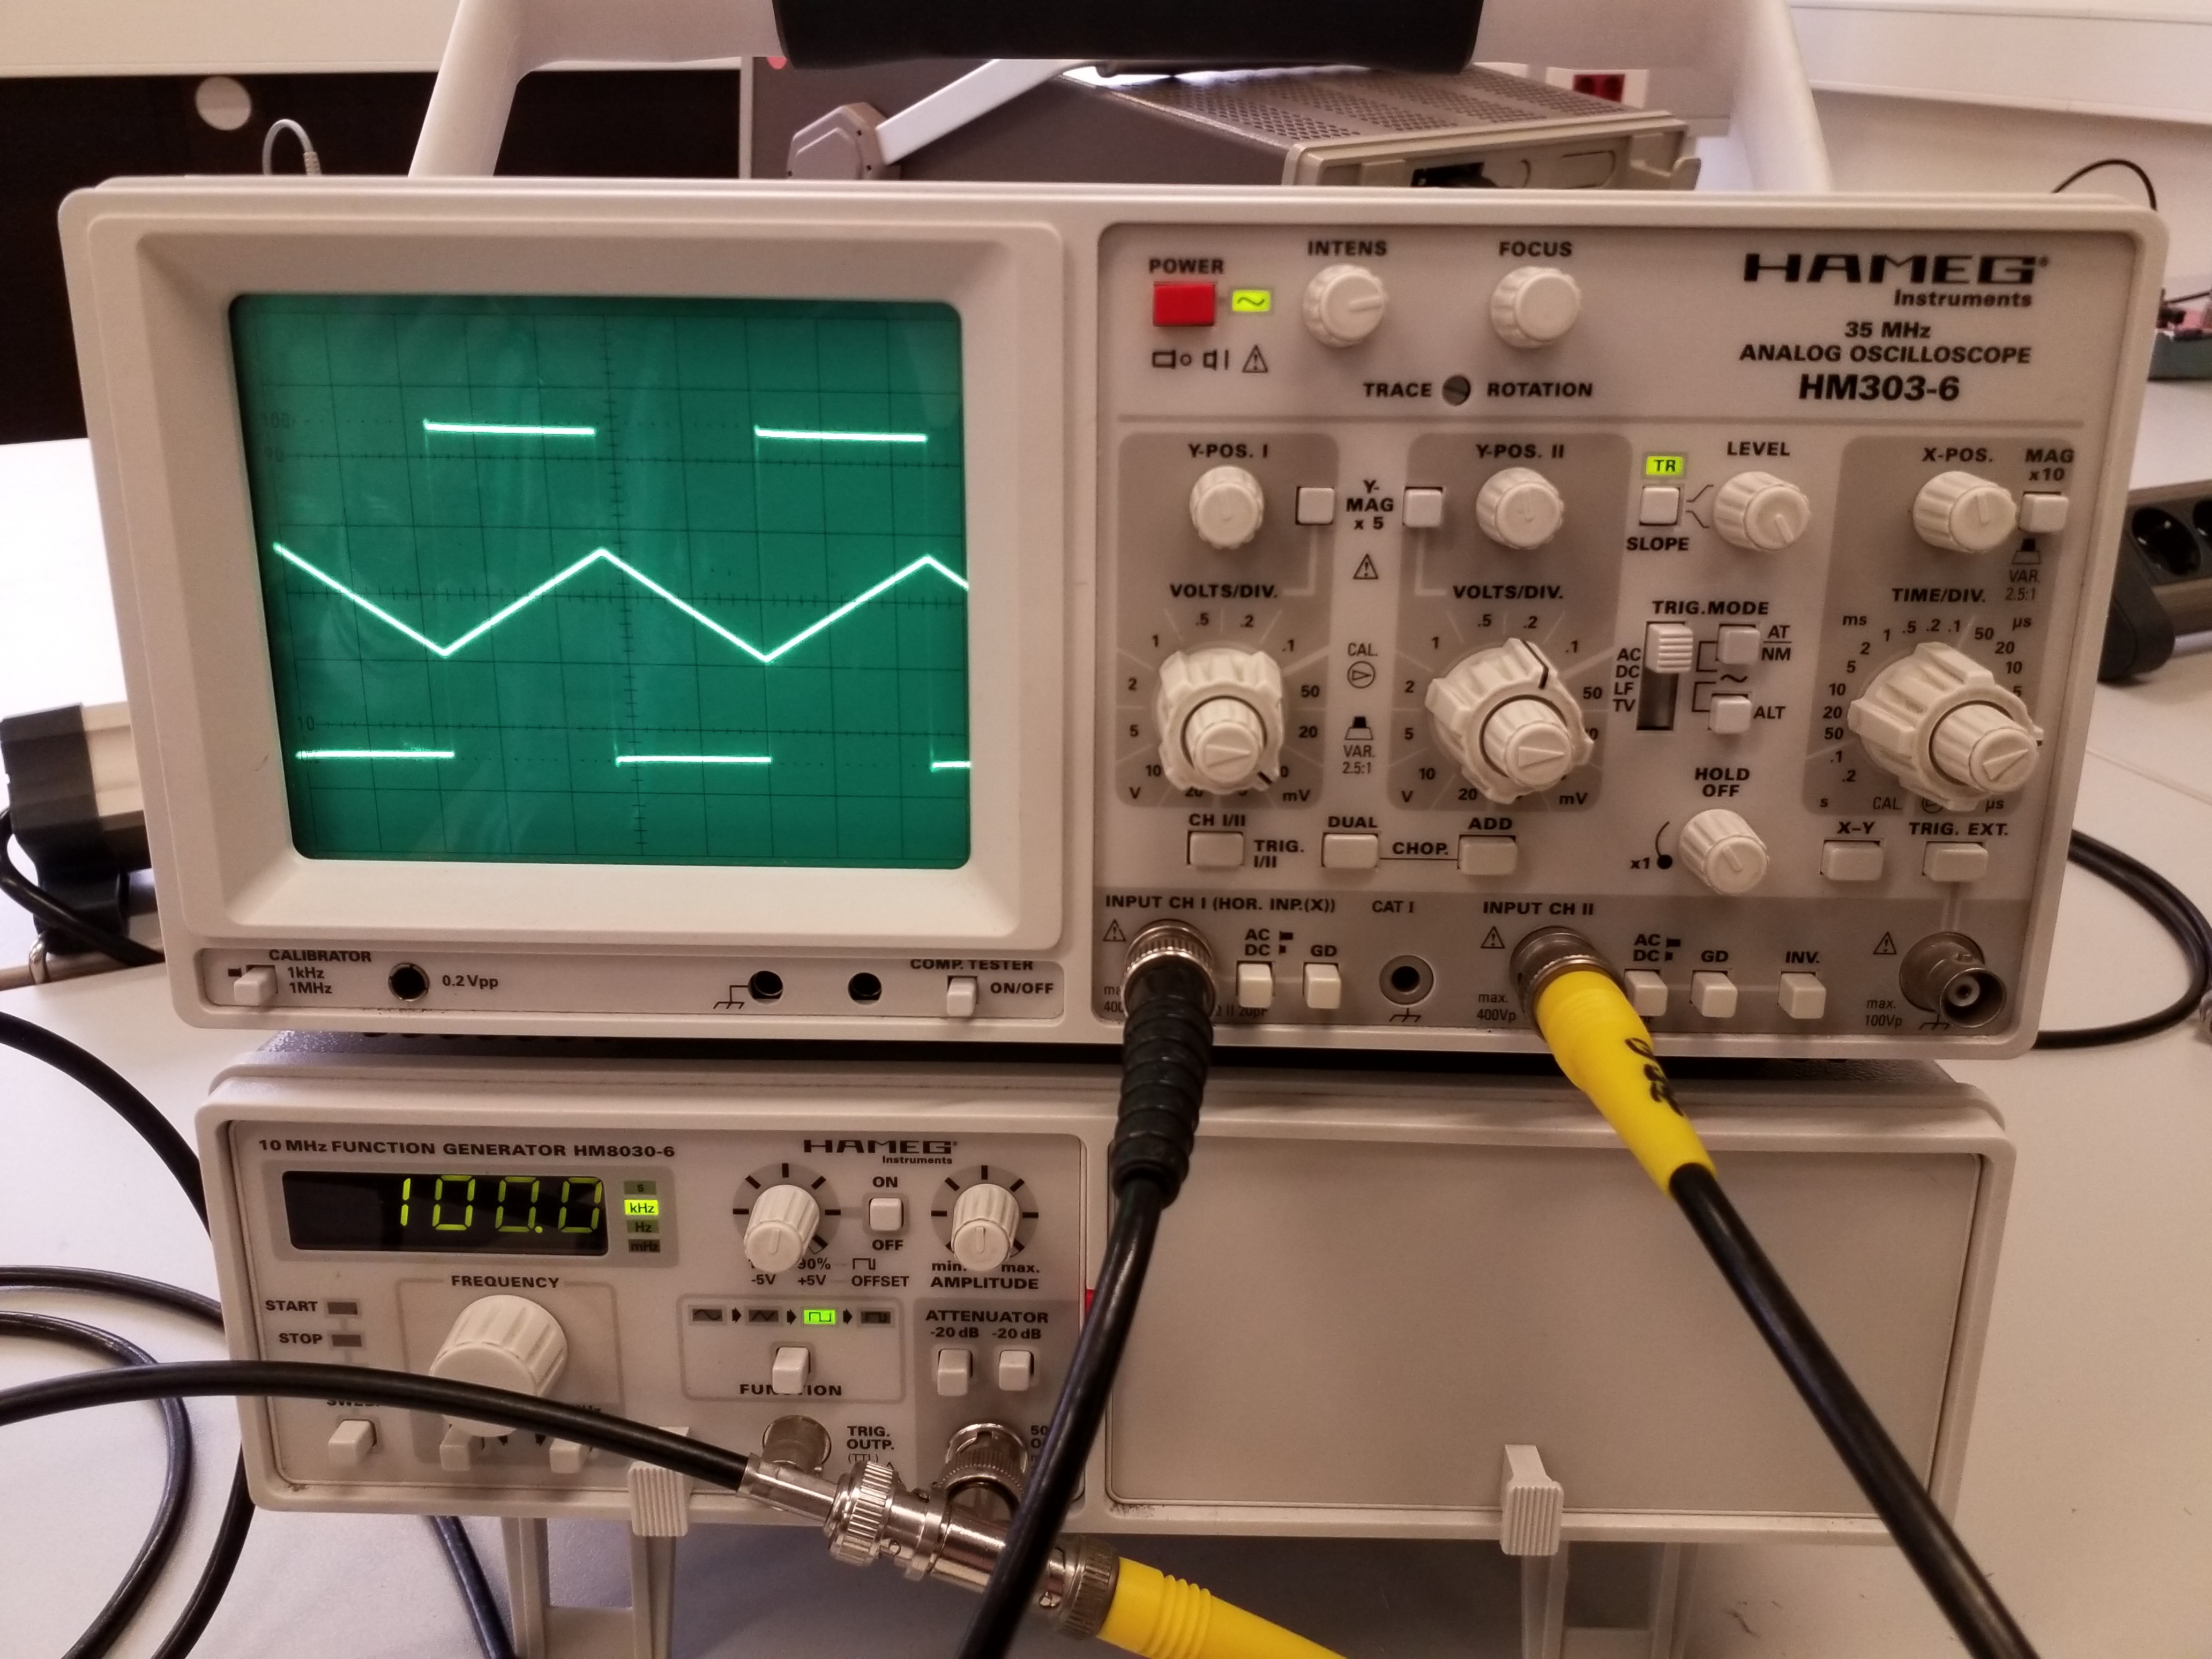
\includegraphics[width=\textwidth]{images/rechteck.jpg}
      \centering
      \caption{Rechteckschwingung für d)}
      \label{fig:rechteck}
    \end{subfigure}
    \begin{subfigure}{0.48\linewidth}
      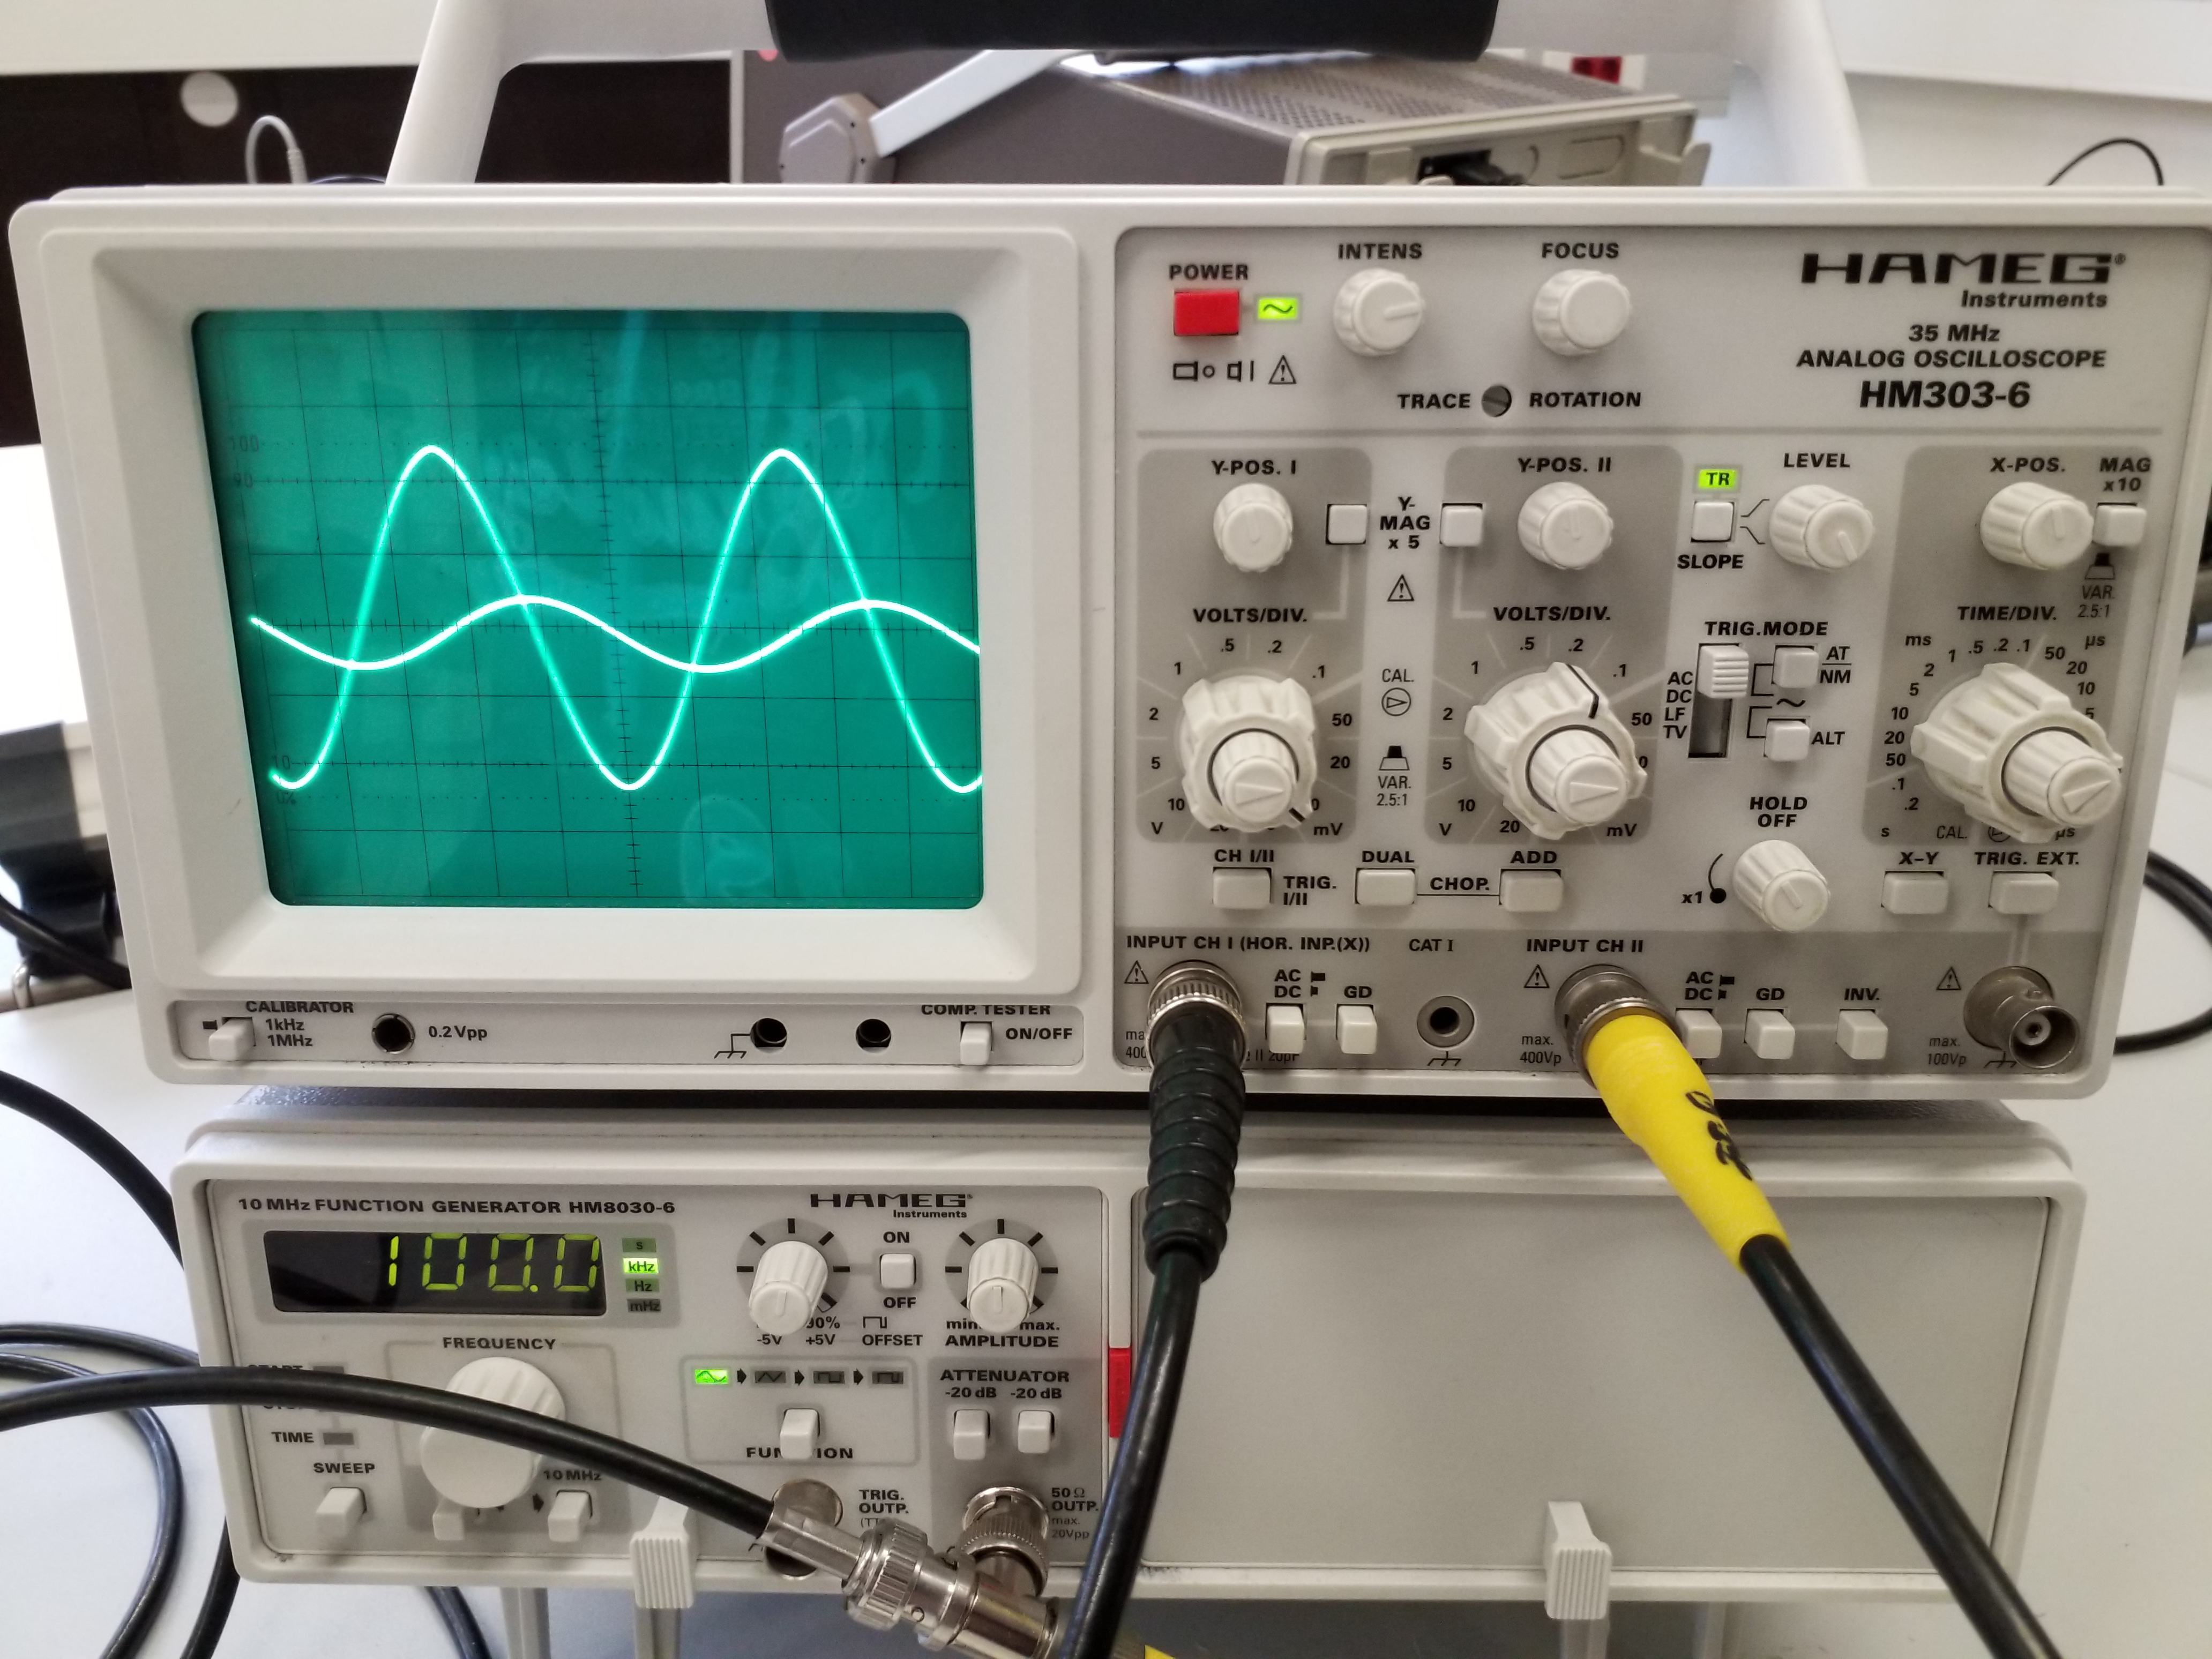
\includegraphics[width=\textwidth]{images/sinus.jpg}
      \centering
      \caption{Sinusschwingung für d)}
      \label{fig:4c}
    \end{subfigure}
    \begin{subfigure}{0.48\linewidth}
      \vspace{5mm}
      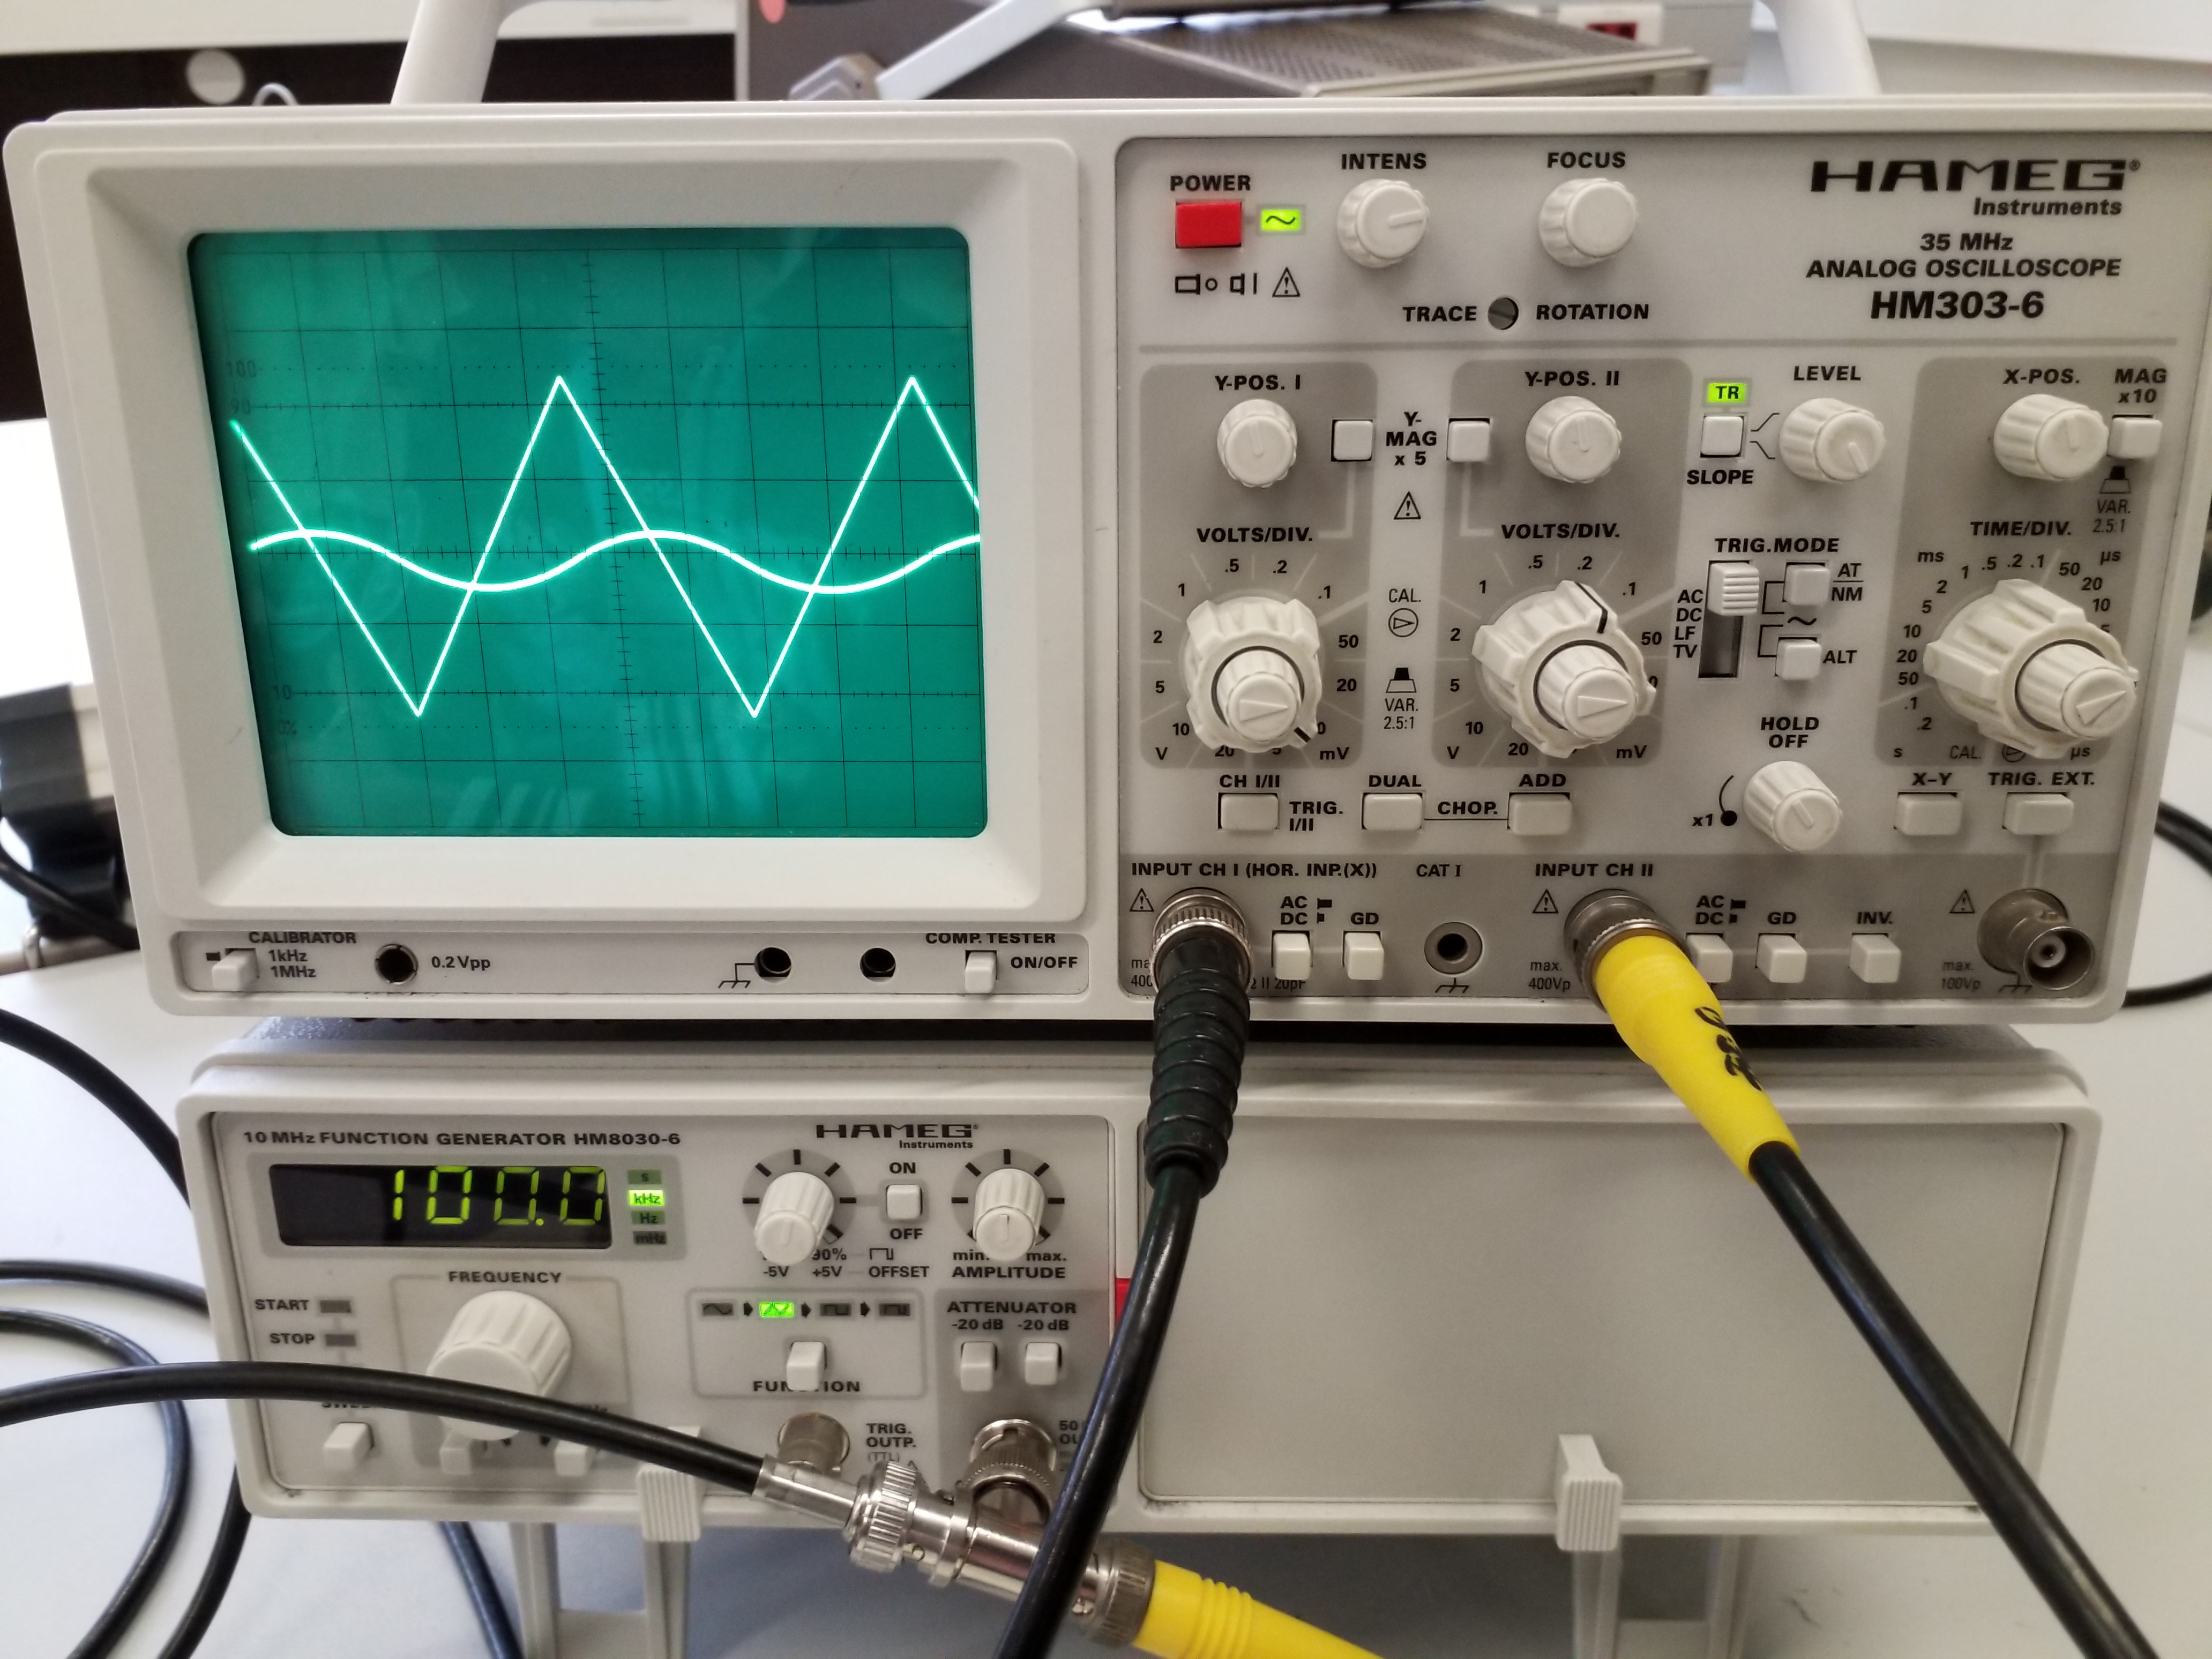
\includegraphics[width=\textwidth]{images/dreieck.jpg}
      \centering
      \caption{Dreieckschwingung für d)}  
    \end{subfigure}
  \end{figure}

  \begin{figure}[H]
    \includegraphics[width=\textwidth]{build/plot4d.pdf}
    \centering
    \caption{Polarplot von Aufgabe d)}
    \label{fig:4d}
  \end{figure}

  


\section{Diskussion}

% Diskussion 4c %%%%%%%%%%%%%%%%%%%%%%%%%%%%%%%%%%%%%%%%%%%%%%%%%%%%%%%%%%%%%%%%%%%%%%%%%%%%%%%%%%%%%%%%%%%%%%%%%%

  \begin{figure}[H]
    \includegraphics[width=\textwidth]{build/plot4ctrue.pdf}
    \centering
    \caption{korregierte Nichtlineare Regression von Aufgabe c)}
    \label{fig:4ctrue}
  \end{figure}

\newpage
\nocite{V353}
\nocite{scipy}
\printbibliography
\end{document}